\documentclass[tikz,border=0mm]{standalone}
\usepackage[utf8]{inputenc}
\usepackage{unicode-math} % for unicode support in math environments
\usepackage{amsmath}
\usepackage{siunitx}
\usepackage{booktabs}
\sisetup{mode=text,range-phrase = {\text{~to~}}, range-units=single, print-unity-mantissa=false}
\usepackage{mhchem}
\usepackage{tikz}



\usepackage{fontspec}

\directlua{
  luaotfload.add_fallback(
  "FallbackFonts",
  {
        "DejaVu Serif:mode=harf;",
        "DejaVu Sans Mono:mode=harf;",
        % we could add many more fonts here optionally!
    }
  )
}

% \setmainfont{CMU Serif}[RawFeature={fallback=FallbackFonts}]
% For PhD thesis
\setmainfont{STIXTwoText}[RawFeature={fallback=FallbackFonts}]
\setmathfont{STIXTwoMath-Regular}[RawFeature={fallback=FallbackFonts}]
\setmonofont{Inconsolata}[RawFeature={fallback=FallbackFonts}]

\begin{document}
\definecolor{backgroundColor}{rgb}{1.0, 1.0, 1.0}

\pagecolor{backgroundColor}


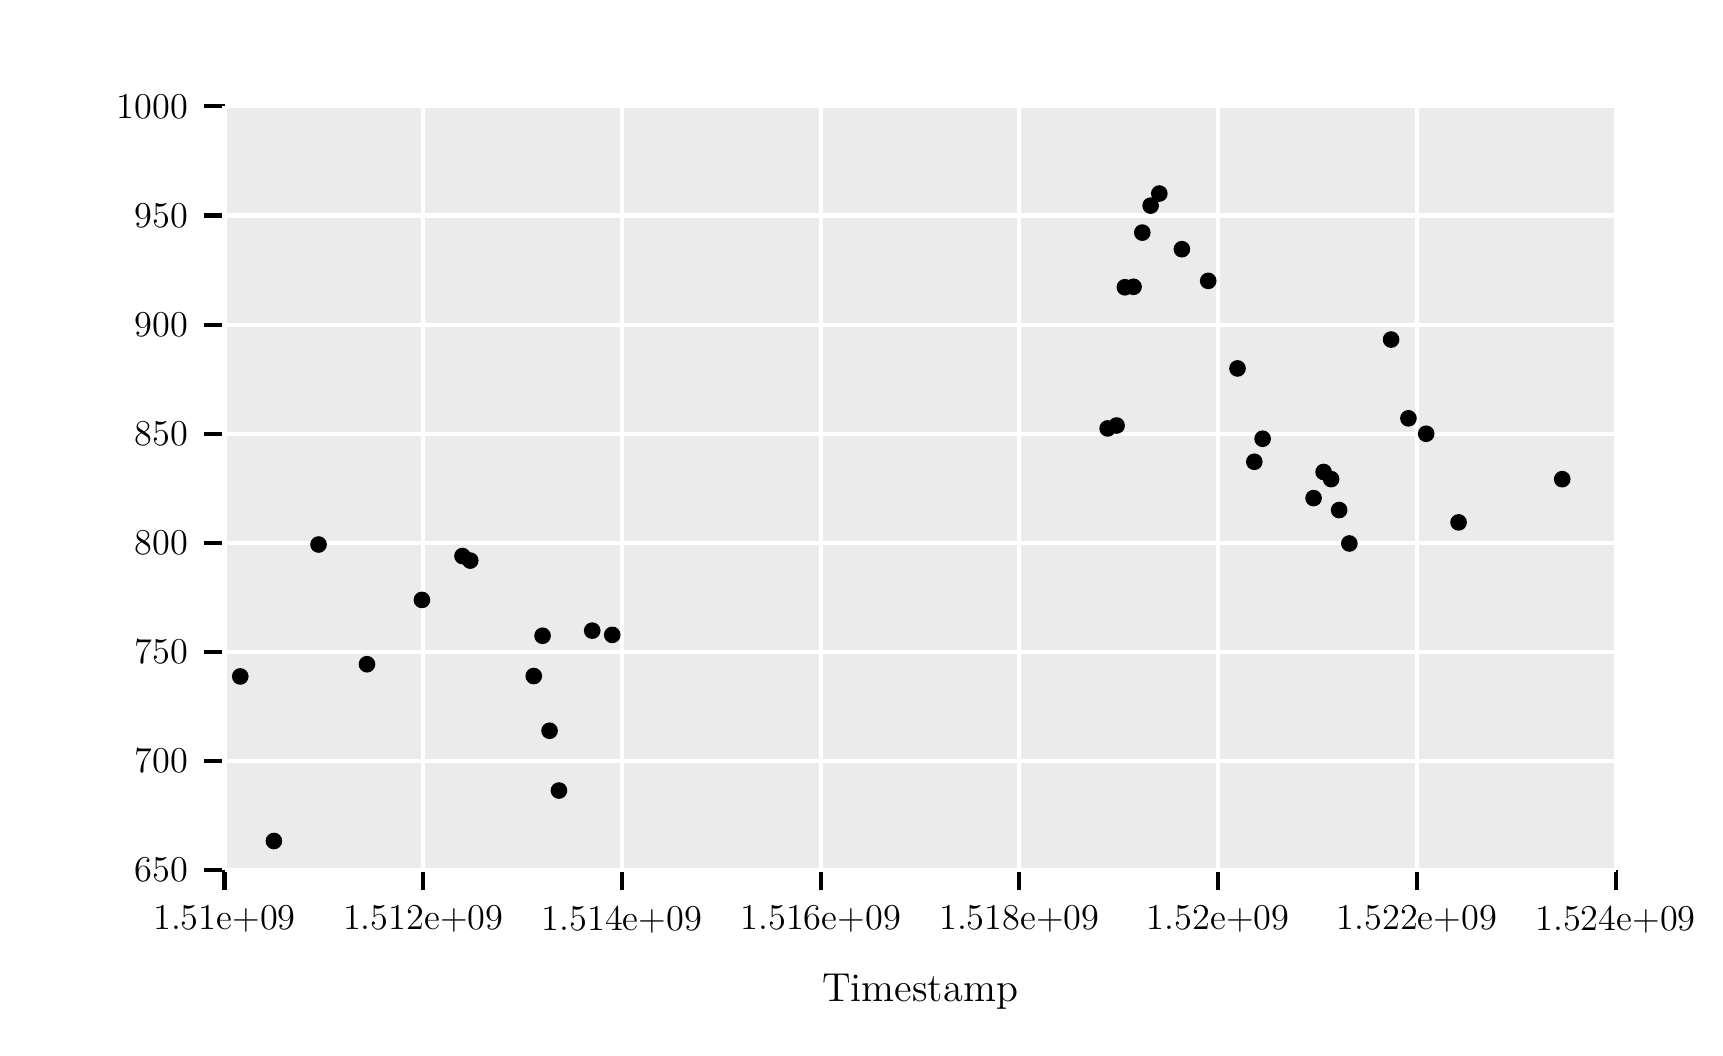
\begin{tikzpicture}[every node/.style={outer sep=0pt, inner sep=0pt}]
\path[use as bounding box] (0, 0) rectangle (600.0bp, 360.0bp) ;
\definecolor{drawColor}{rgb}{0.0, 0.0, 0.0}
\definecolor{fillColor}{rgb}{1.0, 1.0, 1.0}

\draw [color = drawColor, fill = fillColor, draw opacity = 0.0, fill opacity = 1.0, line width = 0.0bp] (0.0000bp, 360.0000bp) rectangle (600.0000bp, 0.0000bp) ;
\definecolor{drawColor}{rgb}{0.0, 0.0, 0.0}
\definecolor{fillColor}{rgb}{0.9200000166893005, 0.9200000166893005, 0.9200000166893005}

\draw [color = drawColor, fill = fillColor, draw opacity = 0.0, fill opacity = 1.0, line width = 0.0bp] (70.8661bp, 331.6535bp) rectangle (571.6535bp, 56.6929bp) ;
\definecolor{drawColor}{rgb}{0.0, 0.0, 0.0}
\definecolor{fillColor}{rgb}{0.0, 0.0, 0.0}

\draw [color = drawColor, fill = fillColor, draw opacity = 1.0, fill opacity = 0.0, line width = 1.46012951083283bp] (70.8661bp, 49.3923bp)--(70.8661bp, 56.6929bp) ;
\draw [color = drawColor, fill = fillColor, draw opacity = 1.0, fill opacity = 0.0, line width = 1.46012951083283bp] (142.4072bp, 49.3923bp)--(142.4072bp, 56.6929bp) ;
\draw [color = drawColor, fill = fillColor, draw opacity = 1.0, fill opacity = 0.0, line width = 1.46012951083283bp] (213.9483bp, 49.3923bp)--(213.9483bp, 56.6929bp) ;
\draw [color = drawColor, fill = fillColor, draw opacity = 1.0, fill opacity = 0.0, line width = 1.46012951083283bp] (285.4893bp, 49.3923bp)--(285.4893bp, 56.6929bp) ;
\draw [color = drawColor, fill = fillColor, draw opacity = 1.0, fill opacity = 0.0, line width = 1.46012951083283bp] (357.0304bp, 49.3923bp)--(357.0304bp, 56.6929bp) ;
\draw [color = drawColor, fill = fillColor, draw opacity = 1.0, fill opacity = 0.0, line width = 1.46012951083283bp] (428.5714bp, 49.3923bp)--(428.5714bp, 56.6929bp) ;
\draw [color = drawColor, fill = fillColor, draw opacity = 1.0, fill opacity = 0.0, line width = 1.46012951083283bp] (500.1125bp, 49.3923bp)--(500.1125bp, 56.6929bp) ;
\draw [color = drawColor, fill = fillColor, draw opacity = 1.0, fill opacity = 0.0, line width = 1.46012951083283bp] (571.6535bp, 49.3923bp)--(571.6535bp, 56.6929bp) ;
\node [font=\fontsize{13.14116559749547}{15.76939871699456}\selectfont
] at (70.8661bp, 39.0441bp){1.51e+09} ;
\node [font=\fontsize{13.14116559749547}{15.76939871699456}\selectfont
] at (142.4072bp, 39.0441bp){1.512e+09} ;
\node [font=\fontsize{13.14116559749547}{15.76939871699456}\selectfont
] at (213.9483bp, 39.0441bp){1.514e+09} ;
\node [font=\fontsize{13.14116559749547}{15.76939871699456}\selectfont
] at (285.4893bp, 39.0441bp){1.516e+09} ;
\node [font=\fontsize{13.14116559749547}{15.76939871699456}\selectfont
] at (357.0304bp, 39.0375bp){1.518e+09} ;
\node [font=\fontsize{13.14116559749547}{15.76939871699456}\selectfont
] at (428.5714bp, 39.0441bp){1.52e+09} ;
\node [font=\fontsize{13.14116559749547}{15.76939871699456}\selectfont
] at (500.1125bp, 39.0441bp){1.522e+09} ;
\node [font=\fontsize{13.14116559749547}{15.76939871699456}\selectfont
] at (571.6535bp, 39.0441bp){1.524e+09} ;
\draw [color = drawColor, fill = fillColor, draw opacity = 1.0, fill opacity = 0.0, line width = 1.46012951083283bp] (70.8661bp, 56.6929bp)--(63.5655bp, 56.6929bp) ;
\draw [color = drawColor, fill = fillColor, draw opacity = 1.0, fill opacity = 0.0, line width = 1.46012951083283bp] (70.8661bp, 95.9730bp)--(63.5655bp, 95.9730bp) ;
\draw [color = drawColor, fill = fillColor, draw opacity = 1.0, fill opacity = 0.0, line width = 1.46012951083283bp] (70.8661bp, 135.2531bp)--(63.5655bp, 135.2531bp) ;
\draw [color = drawColor, fill = fillColor, draw opacity = 1.0, fill opacity = 0.0, line width = 1.46012951083283bp] (70.8661bp, 174.5332bp)--(63.5655bp, 174.5332bp) ;
\draw [color = drawColor, fill = fillColor, draw opacity = 1.0, fill opacity = 0.0, line width = 1.46012951083283bp] (70.8661bp, 213.8133bp)--(63.5655bp, 213.8133bp) ;
\draw [color = drawColor, fill = fillColor, draw opacity = 1.0, fill opacity = 0.0, line width = 1.46012951083283bp] (70.8661bp, 253.0934bp)--(63.5655bp, 253.0934bp) ;
\draw [color = drawColor, fill = fillColor, draw opacity = 1.0, fill opacity = 0.0, line width = 1.46012951083283bp] (70.8661bp, 292.3735bp)--(63.5655bp, 292.3735bp) ;
\draw [color = drawColor, fill = fillColor, draw opacity = 1.0, fill opacity = 0.0, line width = 1.46012951083283bp] (70.8661bp, 331.6535bp)--(63.5655bp, 331.6535bp) ;
\node [left, font=\fontsize{13.14116559749547}{15.76939871699456}\selectfont
, anchor=east] at (57.7483bp, 56.6929bp){650} ;
\node [left, font=\fontsize{13.14116559749547}{15.76939871699456}\selectfont
, anchor=east] at (57.7483bp, 95.9730bp){700} ;
\node [left, font=\fontsize{13.14116559749547}{15.76939871699456}\selectfont
, anchor=east] at (57.7483bp, 135.2531bp){750} ;
\node [left, font=\fontsize{13.14116559749547}{15.76939871699456}\selectfont
, anchor=east] at (57.7483bp, 174.5332bp){800} ;
\node [left, font=\fontsize{13.14116559749547}{15.76939871699456}\selectfont
, anchor=east] at (57.7483bp, 213.8133bp){850} ;
\node [left, font=\fontsize{13.14116559749547}{15.76939871699456}\selectfont
, anchor=east] at (57.7483bp, 253.0934bp){900} ;
\node [left, font=\fontsize{13.14116559749547}{15.76939871699456}\selectfont
, anchor=east] at (57.7483bp, 292.3735bp){950} ;
\node [left, font=\fontsize{13.14116559749547}{15.76939871699456}\selectfont
, anchor=east] at (57.7483bp, 331.6535bp){1000} ;
\node [font=\fontsize{14.6012951083283}{17.52155412999396}\selectfont
] at (321.2598bp, 12.9303bp){Timestamp} ;
\node [rotate = 90.0, font=\fontsize{14.6012951083283}{17.52155412999396}\selectfont
] at (13.1877bp, 194.1732bp){μ} ;
\definecolor{drawColor}{rgb}{1.0, 1.0, 1.0}
\definecolor{fillColor}{rgb}{0.0, 0.0, 0.0}

\draw [color = drawColor, fill = fillColor, draw opacity = 1.0, fill opacity = 0.0, line width = 1.46012951083283bp] (70.8661bp, 331.6535bp)--(70.8661bp, 56.6929bp) ;
\draw [color = drawColor, fill = fillColor, draw opacity = 1.0, fill opacity = 0.0, line width = 1.46012951083283bp] (142.4072bp, 331.6535bp)--(142.4072bp, 56.6929bp) ;
\draw [color = drawColor, fill = fillColor, draw opacity = 1.0, fill opacity = 0.0, line width = 1.46012951083283bp] (213.9483bp, 331.6535bp)--(213.9483bp, 56.6929bp) ;
\draw [color = drawColor, fill = fillColor, draw opacity = 1.0, fill opacity = 0.0, line width = 1.46012951083283bp] (285.4893bp, 331.6535bp)--(285.4893bp, 56.6929bp) ;
\draw [color = drawColor, fill = fillColor, draw opacity = 1.0, fill opacity = 0.0, line width = 1.46012951083283bp] (357.0304bp, 331.6535bp)--(357.0304bp, 56.6929bp) ;
\draw [color = drawColor, fill = fillColor, draw opacity = 1.0, fill opacity = 0.0, line width = 1.46012951083283bp] (428.5714bp, 331.6535bp)--(428.5714bp, 56.6929bp) ;
\draw [color = drawColor, fill = fillColor, draw opacity = 1.0, fill opacity = 0.0, line width = 1.46012951083283bp] (500.1125bp, 331.6535bp)--(500.1125bp, 56.6929bp) ;
\draw [color = drawColor, fill = fillColor, draw opacity = 1.0, fill opacity = 0.0, line width = 1.46012951083283bp] (571.6535bp, 331.6535bp)--(571.6535bp, 56.6929bp) ;
\draw [color = drawColor, fill = fillColor, draw opacity = 1.0, fill opacity = 0.0, line width = 1.46012951083283bp] (70.8661bp, 56.6929bp)--(571.6535bp, 56.6929bp) ;
\draw [color = drawColor, fill = fillColor, draw opacity = 1.0, fill opacity = 0.0, line width = 1.46012951083283bp] (70.8661bp, 95.9730bp)--(571.6535bp, 95.9730bp) ;
\draw [color = drawColor, fill = fillColor, draw opacity = 1.0, fill opacity = 0.0, line width = 1.46012951083283bp] (70.8661bp, 135.2531bp)--(571.6535bp, 135.2531bp) ;
\draw [color = drawColor, fill = fillColor, draw opacity = 1.0, fill opacity = 0.0, line width = 1.46012951083283bp] (70.8661bp, 174.5332bp)--(571.6535bp, 174.5332bp) ;
\draw [color = drawColor, fill = fillColor, draw opacity = 1.0, fill opacity = 0.0, line width = 1.46012951083283bp] (70.8661bp, 213.8133bp)--(571.6535bp, 213.8133bp) ;
\draw [color = drawColor, fill = fillColor, draw opacity = 1.0, fill opacity = 0.0, line width = 1.46012951083283bp] (70.8661bp, 253.0934bp)--(571.6535bp, 253.0934bp) ;
\draw [color = drawColor, fill = fillColor, draw opacity = 1.0, fill opacity = 0.0, line width = 1.46012951083283bp] (70.8661bp, 292.3735bp)--(571.6535bp, 292.3735bp) ;
\draw [color = drawColor, fill = fillColor, draw opacity = 1.0, fill opacity = 0.0, line width = 1.46012951083283bp] (70.8661bp, 331.6535bp)--(571.6535bp, 331.6535bp) ;
\definecolor{drawColor}{rgb}{0.0, 0.0, 0.0}
\definecolor{fillColor}{rgb}{0.0, 0.0, 0.0}

\draw [color = drawColor, fill = fillColor, draw opacity = 0.0, fill opacity = 1.0, line width = 1.0bp] (76.5341bp, 126.4355bp) circle [radius=3.0bp] ;
\draw [color = drawColor, fill = fillColor, draw opacity = 0.0, fill opacity = 1.0, line width = 1.0bp] (88.6444bp, 67.1989bp) circle [radius=3.0bp] ;
\draw [color = drawColor, fill = fillColor, draw opacity = 0.0, fill opacity = 1.0, line width = 1.0bp] (104.7168bp, 173.9299bp) circle [radius=3.0bp] ;
\draw [color = drawColor, fill = fillColor, draw opacity = 0.0, fill opacity = 1.0, line width = 1.0bp] (122.1517bp, 130.8368bp) circle [radius=3.0bp] ;
\draw [color = drawColor, fill = fillColor, draw opacity = 0.0, fill opacity = 1.0, line width = 1.0bp] (141.9331bp, 153.9875bp) circle [radius=3.0bp] ;
\draw [color = drawColor, fill = fillColor, draw opacity = 0.0, fill opacity = 1.0, line width = 1.0bp] (156.5289bp, 169.7731bp) circle [radius=3.0bp] ;
\draw [color = drawColor, fill = fillColor, draw opacity = 0.0, fill opacity = 1.0, line width = 1.0bp] (159.3208bp, 168.1509bp) circle [radius=3.0bp] ;
\draw [color = drawColor, fill = fillColor, draw opacity = 0.0, fill opacity = 1.0, line width = 1.0bp] (182.1963bp, 126.5833bp) circle [radius=3.0bp] ;
\draw [color = drawColor, fill = fillColor, draw opacity = 0.0, fill opacity = 1.0, line width = 1.0bp] (185.3536bp, 141.0865bp) circle [radius=3.0bp] ;
\draw [color = drawColor, fill = fillColor, draw opacity = 0.0, fill opacity = 1.0, line width = 1.0bp] (187.8751bp, 106.8977bp) circle [radius=3.0bp] ;
\draw [color = drawColor, fill = fillColor, draw opacity = 0.0, fill opacity = 1.0, line width = 1.0bp] (191.2613bp, 85.3658bp) circle [radius=3.0bp] ;
\draw [color = drawColor, fill = fillColor, draw opacity = 0.0, fill opacity = 1.0, line width = 1.0bp] (203.2341bp, 142.9219bp) circle [radius=3.0bp] ;
\draw [color = drawColor, fill = fillColor, draw opacity = 0.0, fill opacity = 1.0, line width = 1.0bp] (210.4394bp, 141.3987bp) circle [radius=3.0bp] ;
\draw [color = drawColor, fill = fillColor, draw opacity = 0.0, fill opacity = 1.0, line width = 1.0bp] (388.7913bp, 215.7260bp) circle [radius=3.0bp] ;
\draw [color = drawColor, fill = fillColor, draw opacity = 0.0, fill opacity = 1.0, line width = 1.0bp] (391.9989bp, 216.7682bp) circle [radius=3.0bp] ;
\draw [color = drawColor, fill = fillColor, draw opacity = 0.0, fill opacity = 1.0, line width = 1.0bp] (394.9866bp, 266.5485bp) circle [radius=3.0bp] ;
\draw [color = drawColor, fill = fillColor, draw opacity = 0.0, fill opacity = 1.0, line width = 1.0bp] (398.1020bp, 266.7156bp) circle [radius=3.0bp] ;
\draw [color = drawColor, fill = fillColor, draw opacity = 0.0, fill opacity = 1.0, line width = 1.0bp] (401.2549bp, 286.2165bp) circle [radius=3.0bp] ;
\draw [color = drawColor, fill = fillColor, draw opacity = 0.0, fill opacity = 1.0, line width = 1.0bp] (404.2558bp, 295.9326bp) circle [radius=3.0bp] ;
\draw [color = drawColor, fill = fillColor, draw opacity = 0.0, fill opacity = 1.0, line width = 1.0bp] (407.3847bp, 300.2785bp) circle [radius=3.0bp] ;
\draw [color = drawColor, fill = fillColor, draw opacity = 0.0, fill opacity = 1.0, line width = 1.0bp] (415.5079bp, 280.2533bp) circle [radius=3.0bp] ;
\draw [color = drawColor, fill = fillColor, draw opacity = 0.0, fill opacity = 1.0, line width = 1.0bp] (424.9934bp, 268.8496bp) circle [radius=3.0bp] ;
\draw [color = drawColor, fill = fillColor, draw opacity = 0.0, fill opacity = 1.0, line width = 1.0bp] (435.5332bp, 237.3260bp) circle [radius=3.0bp] ;
\draw [color = drawColor, fill = fillColor, draw opacity = 0.0, fill opacity = 1.0, line width = 1.0bp] (441.5827bp, 203.7185bp) circle [radius=3.0bp] ;
\draw [color = drawColor, fill = fillColor, draw opacity = 0.0, fill opacity = 1.0, line width = 1.0bp] (444.5737bp, 212.0106bp) circle [radius=3.0bp] ;
\draw [color = drawColor, fill = fillColor, draw opacity = 0.0, fill opacity = 1.0, line width = 1.0bp] (462.9153bp, 190.6440bp) circle [radius=3.0bp] ;
\draw [color = drawColor, fill = fillColor, draw opacity = 0.0, fill opacity = 1.0, line width = 1.0bp] (466.5351bp, 200.0427bp) circle [radius=3.0bp] ;
\draw [color = drawColor, fill = fillColor, draw opacity = 0.0, fill opacity = 1.0, line width = 1.0bp] (469.2341bp, 197.4680bp) circle [radius=3.0bp] ;
\draw [color = drawColor, fill = fillColor, draw opacity = 0.0, fill opacity = 1.0, line width = 1.0bp] (472.1299bp, 186.3384bp) circle [radius=3.0bp] ;
\draw [color = drawColor, fill = fillColor, draw opacity = 0.0, fill opacity = 1.0, line width = 1.0bp] (475.7941bp, 174.3053bp) circle [radius=3.0bp] ;
\draw [color = drawColor, fill = fillColor, draw opacity = 0.0, fill opacity = 1.0, line width = 1.0bp] (490.8306bp, 247.7202bp) circle [radius=3.0bp] ;
\draw [color = drawColor, fill = fillColor, draw opacity = 0.0, fill opacity = 1.0, line width = 1.0bp] (497.0734bp, 219.3657bp) circle [radius=3.0bp] ;
\draw [color = drawColor, fill = fillColor, draw opacity = 0.0, fill opacity = 1.0, line width = 1.0bp] (503.4619bp, 213.7996bp) circle [radius=3.0bp] ;
\draw [color = drawColor, fill = fillColor, draw opacity = 0.0, fill opacity = 1.0, line width = 1.0bp] (515.1195bp, 181.9067bp) circle [radius=3.0bp] ;
\draw [color = drawColor, fill = fillColor, draw opacity = 0.0, fill opacity = 1.0, line width = 1.0bp] (552.4322bp, 197.4609bp) circle [radius=3.0bp] ;

\end{tikzpicture}

\end{document}

